\section{Implementation}
The Music Player module consists of a number of classes, where to most notable are \texttt{DynamicQueue}, \texttt{MusicPlayerActivity}, and \texttt{MusicPlayerService}. \texttt{DynamicQueue} handles navigation, and it makes sure the queue of songs matches the user's running speed. \texttt{MusicPlayerActivity} shows a UI on the screen and handles user inputs, including navigation and volume changes. \texttt{MusicPlayerService} handles the actual playback of songs, and because it is implemented as a service it is possible to keep playing songs in the background, i.e., without requiring \texttt{MusicPlayerActivity} to be visible.

\subsection{DynamicQueue}
\label{sec:dynamicQueue}
This class is named based on the fact that it will update dynamically, depending on the runnin speed of the user.

\subsection{MusicPlayerActivity}
This is the central point of the application, responsible for managing the rest of the application and giving the user a way of interacting with it. Is starts the \texttt{MusicPlayerService}, calls the \texttt{DynamicQueue} for songs to play, attaches listeners to the buttons, making them clickable, and it checks that there are enough songs in the specified folder, sending the user to the settings menu if this is not the case.

In order to manage the responsibilities associated with the activity, general initialisation has its own class \texttt{Initializers}. \texttt{Initializers} is responsibility for setting \texttt{OnClickListeners} for the GUI and preparing the first song in the queue and coverflow. 

\subsection{MusicPlayerService} 
This service handles the playing of the music files, this is done with the \texttt{MediaPlayer} class which is part of the \citet{android:MediaPlayer} API. The service is responsible for setting up event listeners and act as an interface to the \texttt{MediaPlayer}.  

We only used of one the two listeners available for the \texttt{MediaPlayer}, the \texttt{OnCompleteListener}. This listener is called when a files reaches its end. In this event the method attracted to the listener selects the next song in Queue, by a \texttt{nextSong} method. \texttt{OnCompleteListener} is also called when an error occur while the \texttt{MediaPlayer} is playing. In our application a illegal state error could happen if one would call \texttt{stop} while the \texttt{MediaPlayer} was not playing, triggering the \texttt{OnCompleteListener} and changing the song to the next in the queue. This was resolved in \texttt{MusicPlayerService} by ignoring \texttt{stop} or other calls if the \texttt{MediaPlayer} was in the wrong state. The \texttt{MediaPlayer}'s state diagram can be seen in \cref{fig:medaiPlayerState}.

\begin{figure}[h!]
  \centering
    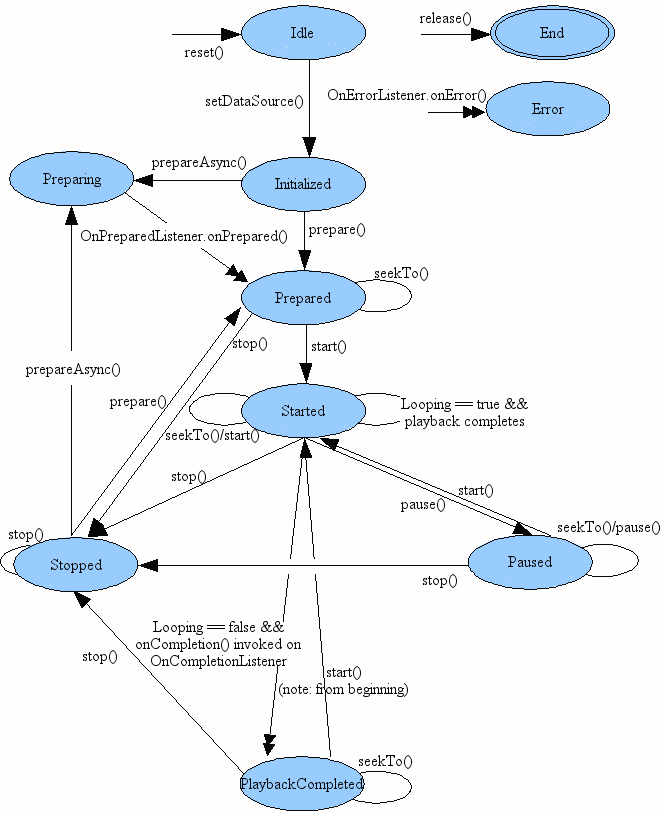
\includegraphics[scale=.33]{Images/mediaplayerStateDiagram.png}
  \caption{A state diagram taken from \citet{android:MediaPlayer}.}
  \label{fig:medaiPlayerState}
\end{figure}
